\documentclass[a4paper, 12pt]{article}
\usepackage[utf8]{inputenc}
\usepackage{subfig}
\usepackage[ngerman]{babel}
\usepackage{amsmath,amsfonts,amssymb}
\usepackage{csquotes}
\usepackage{syntax}
\usepackage{minted}
\usepackage{lmodern}
\usepackage[T1]{fontenc}
\usepackage{wrapfig}

\usepackage{graphicx}
\graphicspath{{./images/}}

\usepackage[margin=3.5cm]{geometry}

\usepackage[
    backend=biber,
    style=numeric,
    sortlocale=de_DE,
    url=true,
    eprint=false,
]{biblatex}
\addbibresource{ref.bib}

\usepackage[]{hyperref}
\hypersetup{
    colorlinks=true,
    citecolor=black,
    urlcolor=blue,
    linkcolor = black
}

\pagenumbering{gobble}

\begin{document}

\clearpage
\tableofcontents
\clearpage

\pagenumbering{arabic}

\section{Vorwort}
Eine vollständige Version des Projektes inklusiver dieser Ausarbeitung können sie online unter folgender Adresse finden: https://github.com/Crypec/Stegi

\section{Aller Anfang ist schwer (Leonie Zumsteg)}
Wir machten uns schon Anfang Mai 2019 Gedanken um den Seminarkurs des nächsten Schuljahres. Wir waren motiviert und suchten nach einer guten Projektarbeit, hierbei wollten wir den größtmöglichen Erfolg erzielen. Das größte Problem bei der Findung eines geeigneten Projekts lag bei dem Zusammenfluss von GGK/Ethik und Informatik. Gerade hier machten wir uns viele Gedanken, da wir schlussendlich ein Prüfungsfach mit dem Seminarkurs ersetzen wollten. Wir merkten schnell das dies nicht leicht werden wird und entschieden uns kurzfristig für ein Technisches Projekt. Nach vielen verschieden Ansätzen kamen wir auf die Idee, eine eigene Programmiersprache für Anfänger zu kreieren. Wir wussten aus eigener Erfahrung von den Problemen als Programmieranfänger und es schien sinnvoll zu helfen, um anderen den Einstieg zu erleichtern. Zu diesem Zeitpunkt wussten wir, dass dieses Projekt nicht in ein paar Monaten umsetzbar ist. Aus diesem Grund fiel das Technische Projekt ins Wasser und wir entschlossen uns erneut für den Seminarkurs. Diesmal aber mit der Entscheidung kein Prüfungsfach damit ersetzen zu können, da wir für dieses Projekt nur Software (ITS) benötigten. 
Unser Projekt nahm Fahrt auf im Sommer 2019, wir sind motiviert und begeistert gestartet, aber wir wussten auch was für eine Herausforderung vor uns liegt. Da Torben und Ich noch nicht lange in der „Informatik-Welt“ waren, hatten wir großen Respekt vor dem Projekt und der Umsetzung. Es gab viele Möglichkeiten der Umsetzung und es dauerte einige Zeit bis wir uns sicher waren wie und in welcher Sprache wir das Projekt angehen und umsetzen werden (obwohl sich auch hier noch viel geändert hat). Vor allem das Ziel des Projekts hat uns gefallen, denn es war noch sehr präsent, welche Fehler man als blutiger Anfänger macht. Der Gedanke anderen somit zu helfen, empfanden wir als motivierend und sinnvoll. 
Der Anfang von 12.1 war auch der aktive Anfang unserer Projektarbeit. Wir fingen an mit der Aufgabenverteilung, welche schlussendlich nicht 100\% aufging, da wir vieles gemeinsam durchgeführt haben und gewisse Aufgaben wegfielen bzw. dazu kamen. Um unser Zeitmanagement einzuhalten hatten wir ein Gantt-Diagramm erstellt und es versucht so gut wie möglich anzupassen und zuführen. 10 Monate später kann ich sagen, dass es für uns umständlicher war es anzupassen als ohne Gantt-Diagramm weiterzumachen. Dennoch konnten wir gut den erstellen Zeitplan einhalten.  

\section{Zeitplanung}
Wir haben die Zeit am Freitagnachmittag immer gut genutzt und unsere Arbeit hauptsächlich auch dort verrichtet. Oftmals sind wir bis um 17Uhr geblieben, da es uns am Sinnvollsten erschien Zeit mit der Gruppe zu nutzen, um Sachen zu besprechen, anstatt miteinander zu telefonieren. Wir waren produktiv, dennoch zog sich das Projekt die ersten Wochen hin und wir gerieten minimal aus dem Zeitplan. Dies holten wir aber wieder ein, als jeder schlussendlich mit dem Projekt vertraut war und wusste was er zu tun hatte. Eine größere Herausforderung war dann die Corona-Krise, da wir nun alle selbstständig von zuhause weitermachen mussten, fiel es uns schwieriger anzufangen, da man das Arbeiten in der Gruppe gewöhnt war. Wir hielten dennoch wöchentliche Anrufe, um unseren Fortschritt zu sammeln und ggf. Probleme zu besprechen. Wir hatten Glück, da unser Projekt hauptsächlich am PC stattfand und wir nicht auf das Dasein in der Schule angewiesen waren. Dennoch wäre es schön gewesen zusammen am Projekt zu arbeiten. Andere Gruppen hatten hier viel größere Schwierigkeiten und konnten teilweise nicht weitermachen. Auch hier kamen von der Schule leider keine Infos und Termine. Die Gruppen waren auf sich allein gestellt, trotzdem waren unsere Fachbereich Lehrer immer für uns erreichbar.  Uns wurde zugesagt, dass rechtzeitige Infos rausgegeben werden, da wir nicht wussten wann die Termine der neuen Abgaben sind und wie es weitergeht. Schlussendlich wurden uns die Termine der Abgabe nur 8 Tage zuvor gesagt. Diese Zeit empfanden alle Teilnehmer des Seminarkurses als sehr kurz und nicht als rechtzeitig. Der Zeitdruck stieg, da man eine Woche zuvor nicht zu 100\% wusste, wann was weitergeht. Genau deshalb wäre eine rechtzeitige Info (2 bis 3 Wochen vorher) für sehr viele Hilfreich gewesen. Wir haben weiterhin vor an unserem Projekt, unabhängig von der Schule weiterzumachen und somit auch weitere Arbeitsblätter zu erstellen und das Programm zu optimieren.

\subsection{Teamgeist (Leonie Zumsteg)}
Als Team haben wir sehr gut zusammen funktioniert, denn es war ständig lustig, wir hatten gute Ideen, jeder gab konstruktive Kritik und so funktionierte das Projekt schlussendlich auch. Wir arbeiteten sehr oft zusammen, hierbei gefiel nicht immer jedem alles, aber Kompromisse fanden wir immer. Vermutlich hatten wir mehr Spaß an diesem Projekt als viele andere, da jeder etwas gemacht hat ohne, dass man ihn täglich dazu auffordern musste. Grundsätzlich kann ich sagen, dass ich selten in einer so eigenständigen und produktiven Gruppe gearbeitet habe. 

Das Gantt-Diagramm (Leonie Zumsteg)
Das Gantt-Diagramm ist ein gängiges Diagramm für das Projektmanagement, um Aktivitäten, Termine und Deadlines einzutragen. Grundsätzlich sollte uns das Gantt-Diagramm helfen unsere Aufgaben rechtzeitig fertig zu bekommen und wenn nötig, mehr Zeit einzuplanen. Leider war es sehr schwer, die Zeit gegen Ende einzuplanen, da wir sehr lange nicht wussten wann der Abgabetermin ist.

\begin{figure}
    \caption{Jahresr\"uberblick unserer Projektplanung}
    \centering
    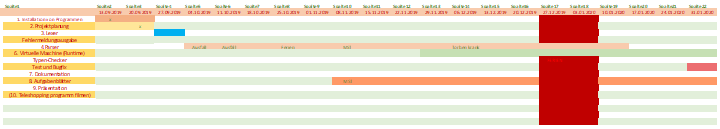
\includegraphics[scale=0.6]{gantt1}
\end{figure}
\begin{figure}
    \centering
    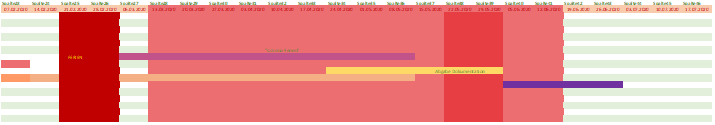
\includegraphics[scale=0.6]{gantt2}
\end{figure}

Die Idee ein Diagramm zu führen war hilfreich, doch wir merkten nach ein paar Monaten, dass es sinnvoller gewesen wäre für jeden zusätzlich ein eigenes zuführen. Dennoch haben wir wöchentlich das Diagramm angepasst und wichtige Daten eingetragen. Wöchentliche Planungen waren wichtig und wir wussten, wenn wir aus dem Zeitplan gerieten (positiv als auch negativ) und wie wir diese Zeit anderweitig nutzen konnten.  Für uns als Team, war das Gantt-Diagramm eine nette Hilfestellung aber nicht unbedingt notwendig. Wir hätten auch gut ohne diese Planung die zeitlichen Deadlines und Meilensteinsitzungen einhalten können. Bei meinem nächsten Projekt würde ich es in Betracht ziehen nochmal eins zuführen, dann aber zusätzlich ein eigenständiges, welches man aktiv auf sich selbst anpasst. 

\section{Der pädagogische Aspekt des Projekts}
\subsection{Ziel des Projekts}
Ziel ist es, Anfängern das Programmieren leichter zu machen. Wir wussten genau welche Schwierigkeiten Anfänger haben, da die eigenen Probleme vom vergangenen Jahr noch sehr präsent waren. Typisch Anfänger: Klammern werden nicht geschlossen, Befehle werden nicht richtig benutzt bzw. geschrieben, Semikolons werden vergessen etc. Und genau für diese kleinen, aber fatalen Probleme wollten wir Abhilfe schaffen. Beim Lernen sind auch eindeutige und hilfreiche Fehlermeldung notwendig. Vor allem in Java, fehlen eindeutige Fehlermeldungen und es kann schon vorkommen, dass man 2 Stunden seinen Fehler sucht, genau das wollten wir bei STGI vermeiden!  Denn langes Suchen, verdirbt einem den Spaß und der Lernfaktor ist gering.  Dazu erzählt Torben mehr.
Um Lernen zusätzlich so leicht wie möglich zu machen, kreieren wir Arbeitsblätter und Hinführungen für das Programmieren. Wir wussten, welche Fehler man als Anfänger macht und wie nervig es sein kann, diese zu beheben. Programmieranfänger werden zwar nie fehlerfrei sein, (Fehlerfrei zu sein ist auch nicht das Ziel, denn vor allem beim Programmieren lernt man durch seine eigenen Fehler) aber wir versuchten, einige Begriffe und Einstiege zu vereinfachen. Hierfür nutzten wir Literatur aus einem Kinderbuch für Einsteiger in die Welt des Programmierens. 

\subsection{Wie macht man eine Programmiersprache lernfreundlich?}
STGI ist eine deutsche Programmiersprache und wir hoffen, dass viele Anfänger besser durch die deutschen Befehle lernen können. Ziel war es, dass das Lernen mit STGI einfacher ist, als mit einer englischen Programmiersprache. Das war der allererste Grundsatz, den wir für unserer Projekt hatten, denn wir vermuteten, dass es in Deutsch für Einsteiger einfacher sein wird.
Es fing an mit der Syntax Planung, hiermit starteten wir Ende September 2019. Wir steckten sehr viel Planung hinein, denn es war wichtig, wie leicht man sich die Befehle schlussendlich merken konnte und wie groß der Lerneffekt dabei ist. Den Syntax haben wir sehr einheitlich gestaltet egal ob Variable, Funktion oder Schleife, denn es ist wichtig einen roten Faden beim Lernen beibehalten zu können.  
Wir versuchten die Befehle so verständlich wie möglich zu benennen, deshalb veränderten wir im Laufe das Jahres immer wieder den Syntax, da viele neue und gute Ideen dazukamen. 
Man lernt leichter, wenn man sich aus dem Namen eines Befehls die jeweilige Tätigkeit erschließen kann und genau das haben wir versucht zu erreichen. Wir haben die Befehle so gut wie möglich übersetzt, damit der Anfänger die Tätigkeit des Befehls erschließen oder zumindest vermuten kann. Trotz Vereinfachung der Befehle, kommt man nicht drumherum die Theorie zu lernen. Sie ist mit das wichtigste, um den Grundbaustein für das Verständnis eines Programms zulegen. Genau aus diesem Grund haben wir uns für die Aufgabenblätter entschieden. 
Die Aufgabenblätter haben wir auf keine bestimmte Altersgruppe ausgelegt, Hauptziel war es, dass sie so einfach und verständlich wie möglich sind, ohne dass ein Lehrer benötigt wird. (Die Grundlagen des Programmierens muss man, dennoch können, hierfür haben wir keine Abhilfe geschaffen)

\begin{figure}
    \caption{Beispiel der Markdownoberflaeche}
    \centering
    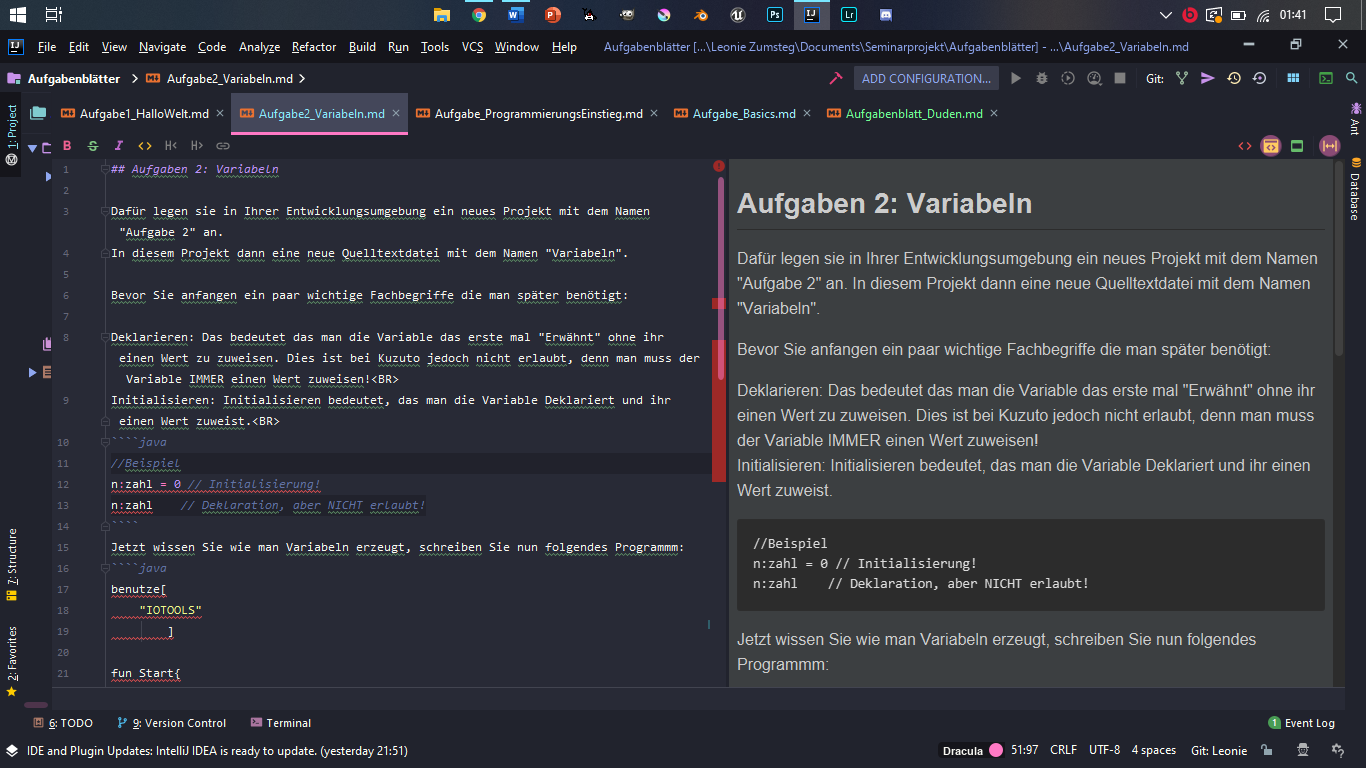
\includegraphics[scale=0.3]{md}
\end{figure}

Bei den Aufgabenblättern war uns wichtig, die Aufgabenstellung so leicht wie möglich zu halten. Hierbei orientierten wir uns an den Arbeitsblättern von Herr Verderber, da diese uns gut gefielen und wir das Jahr zuvor Java damit gelernt hatten. Wir entschieden uns die Arbeitsblätter mit Markdown zu schreiben, denn dies ähnelt HTML sehr und bestimmte Code-Abschnitten waren schön eingerückt und formatiert. 
Dies wäre nicht so schön geworden, hätten wir es in Word verfasst. Außerdem war es möglich bestimmte Formatierung einzubauen, ohne in der Menüleiste danach suchen zu müssen.
Die Arbeitsblätter sind relativ kurzgehalten, damit der Spaßfaktor erhalten bleibt. Dennoch sind sie so ausgelegt, dass man immer ausprobieren kann wo die Grenzen des Programms liegen. Experimentieren ist hierbei gewünscht und gefordert, denn nur so kann man nachhaltig lernen und austesten weshalb manche Sachen in der Informatik so sind wie sie sind. Dennoch sind die Arbeitsblätter großer Aufwand, da viel Planung in ihnen steckt und wir es so einfach wie möglich halten wollten.
Wie wir wissen kann die Sprache in der Informatik sehr komplex sein und man lernt sehr viele neue Begriffe, die man schnell verwechseln kann. Deshalb haben wir zusätzlich und unabhängig von STGI einen kleinen „Programmier-Duden“ erstellt, um sprachliche Konflikte zu vermeiden. Dies kann sehr hilfreich sein, denn viele Begriffe muss man richtig verwenden können, ohne sie durcheinander zu bringen. 
Das waren die Ideen, die wir benutzt haben, um „STGI“ Anfängergerecht zumachen. Wir werden weiterhin daran arbeiten, vor allem um weitere Arbeitsblätter zu erstellen und den Syntax ggf. zu verändern, sobald es Tester für unser Projekt gibt. An den Testern können wir dann feststellen wie gut der Lerneffekt wirklich ist. Die Arbeitsblätter werden stetig ausgebaut und vervollständigt, bzw. erweitert. Es werden weitere Aufgabenblätter folgen, die wir geplant haben, aber zu denen wir noch nicht kamen, da die Zeit knapp wurde. 

\subsection{Namensfindung}
Die Namensfindung war ein sehr schwieriger Teil für uns, da uns vieles nicht gefallen hat und wir uns ständig umentschieden. Anfangs hatten wir die Sprache „Zuse“ und den Compiler „Konrad“ genannt, dies war ein Honorar an Konrad Zuse, denn ohne ihn wären wir nicht dort wo wir heute sind. Trotz des originellen Namens entschieden wir uns um und wir machten Gedanken für einen neuen Namen. Wir wussten, dass dies nicht das dringendste Problem ist und somit verschoben wir die Aufgabe der Namensfindung ans Ende des Schuljahres. Die erste gute Idee nach einer längeren Zeit, welche allen gefallen hatte, war „Kuzuto“. Dieser Name war aber ziemlich langweilig da wir einfach nur versucht hatten, einen Namen zu kreieren, indem wir die Anfänge unserer Namen aneinanderreihten. Wir blieben für einige Monate dabei bis uns etwas anderes einfiel. 
Da wir als Logo/Maskottchen ein Tier wollten, suchten wir erstmal nach einem Tier, welches uns am besten gefiel. Die Ideen waren endlos aber nie passend und irgendwer hatte immer etwas auszusetzen. Dann hatten wir die Idee mit dem Drachen des Compilerbuchs. Somit kamen wir auf den Stegosaurus, diese Idee gefiel allen und ich erstellte die ersten Skizzen für das Logo. 
Als das Logo fertig war änderten wir den Namen in „Stegi“. Nach einigen Wochen fiel uns etwas auf - in „Stegi“ steckten die Initialen für „Technisches Gymnasium Informationstechnik“ Wegen diesem Zufall entschieden wir uns dann final für den Namen „STGI“. Hiermit waren alle zufrieden und nach 9 Monaten stand der Name dann endgültig fest.

\subsection{Logo- und Banner-Design}
Kurz nachdem wir eine Grundidee für den Namen unserer Sprache gefunden hatten, ging es an das Logo/Banner-Design. Zu einem fertigen Produkt gehört schließlich auch der äußerliche Aspekt. Wir benötigten vor allem einen Banner/Logo für das GIT-Projekt. 
Zu diesem Zeitpunkt hatte ich kein eigenes Grafik-Tablet, dies stellte sich als Problem heraus, da wir das Logo in guter Auflösung benötigten. Der Banner konnte nicht traditionell gezeichnet werden und wir waren auf ein Tablet angewiesen. Ich erfuhr, dass die Schule ein neues Wacom Cintiq 22HD hatte (der Maserati unter den Tablets) und somit war mein Problem gelöst.

\begin{figure}[h]
    \caption{Runde Version unseres Logo f\"ur Applikationsicons}
    \centering
    
\includegraphics[scale=0.3]{logo-round}
\end{figure}

In das Logo gingen viele Gedanken hinein, da wir einen richtigen Bezug zu unserem Projekt haben wollten und nicht nur etwas, was uns optisch anspricht. Da wir durch den Stegosaurus auch auf den Namen kamen, lag es nah was das Logo schmücken wird. Es stellte sich heraus, dass auch Herr Verderber ein großer Fan des Stegosaurus war und wir hatten somit die finale Grundidee für das Design. 


Dennoch wollten wir, dass der eigentlich „gefährlich“ ausschauende Dinosaurier, freundlich und einladend aussieht. Die spitzen Rautenförmigen Rückenplatten wurden mit Runden Platten ersetzt, um einen eine freundliche Stilisierung zu erzielen.  
Da wir uns mit Compilern beschäftigten, erinnerten wir uns an das Buch „Compiler: Prinzipien, Techniken und Werkzeuge“ geschrieben von Alfred V. Aho, Monica S. Lam, Ravi Sethi und Jeffrey D. Ullman. Es wurde 1986 veröffentlicht und gilt seitdem als klassischer Compilertechnologietext. Der Buchinhalt ist hierbei nicht so wichtig, sondern das Aussehen, besser gesagt das Cover dieses Klassikers. 

\begin{figure}
    \caption{Cover des Drachenbuches}
    
\includegraphics[scale=0.2]{dragon-book}
\end{figure}

Wir wollten diesen Drachen in unseren Banner mit einbeziehen, da wir diesen Klassiker ehren wollten, indem wir ein sogenanntes „Easter-Egg“ einbauten. Auch hier haben wir den Stil verändert und somit einen sehr harmlosen „Compiler-Dino“ kreiert. Der Banner sieht schlussendlich sehr freundlich und ansprechend aus, genau das, was uns gut gefiel. 

\begin{figure}[h]
    \caption{Das fertige Logo}
    \centering
    
\includegraphics[scale=0.3]{logo-big}
\end{figure}

\section{Meine Erfahrungen und Gedanken über den Seminarkurs}
Die Meinungen über den Seminarkurs gehen sehr weit auseinander, von großer Begeisterung zu purer Abneigung. Ich persönlich war nie wirklich abgelehnt, aber begeistert war ich auch nicht. Als wir dann unser finales Thema abgegeben haben, kam die Motivation und Vorfreude ein solches Projekt umzusetzen. Die Stunden am Freitagmittag haben Spaß gemacht und wir haben produktiv gearbeitet.  Die Zeit verflog schnell und wir blieben meistens bis halb 5 oder 5 Uhr in der Schule. Wir arbeiteten sehr aktiv an unserem Projekt, somit hielten wir den Zeitplan ein und man wusste, dass man die Abgaben und Meilensteine pünktlich schafft.
Im Januar/Februar wurden dann die Technischen Projekte abgeben, das hieß für uns so viel wie „Halbzeit“. Wir merkten, dass unser Projekt selbst fast fertig sein sollte, da im Mai die Abgabe der Dokumentation war. 
Wenige Wochen später, wurden dann die Schulen geschlossen und die wöchentlichen Schulstunden fielen weg. Zuhause war die größte Herausforderung die Arbeit anzufangen und konzentriert zu bleiben. Ich persönlich hatte die ersten Wochen Schwierigkeiten damit. Als diese Phase überwunden war arbeiteten wir selbstständig weiter. 
Schlussendlich kann ich sagen, (Stand: Mitte Juni) dass ich den Seminarkurs empfehlen würde, wenn man das Ziel hat ein Prüfungsfach damit zu ersetzen. Für das Profilfach Informatik ist es schwieriger GGK oder Ethik einzubauen, als für andere Profilfächer, die zusätzlich etwas Bauen können. Es ist eine gute Erfahrung, wenn man gerne länger an etwas arbeitet und somit ein größeres Projekt auf die Beine stellen möchte. 
Covid-19 hat unserem Jahrgang viele Umstellungen beschert. Vor allem im Bereich des Seminarkurses hatte niemand Informationen für uns und deshalb wussten wir auch nicht wie es weitergeht und wann die einzelnen Termine sind. Das sehe ich als großen Minuspunkt, da die Infos vom Kultusministerium sehr spät kamen und wir uns an niemand wenden konnten, da auch kein Lehrer etwas neues wusste. 
Viele Gruppen konnten nicht weiterarbeiten, da die Projekte in der Schule waren oder sie eine Werkstatt benötigten. Diesen Gruppen fehlen jetzt Wochen an Arbeit, diese Zeit können sie auch nicht aufholen, da nicht genug Zeit nach der Schulöffnung gegeben wurde. 
Der Seminarkurs ist eine großartige Chance sein Abitur zu verbessern, dennoch würden einige Korrekturen und Verbesserungen den Seminarkurs attraktiver machen. Viele Schüler sehen den Seminarkurs als Last und viel Arbeit an. Arbeit, welche sich schlussendlich nicht lohnt, da man nicht sofort weiß ob man eine Prüfung ersetzen kann oder nicht. Dies empfinde ich nicht so, da man wirklich großartige Projekte auf die Beine stellen kann und mit der richtigen Gruppe einiges erreicht. 

\section {Vorwort(Torben Grötzinger)}
Am Anfang waren wir sehr unschlüssig, ob wir uns sicher sind, zusammen eine drei-er Gruppe zu bilden. Das war der Grund, weshalb wir uns auch sehr oft über The-men unterhalten haben, die uns interessierten. Wir wollten sehen, wie wir harmonie-ren oder unsere einzelnen Sichtweisen zu bestimmten Themen oder Projektvor-schlägen austauschen. Nach 3 Wochen und Vorschlägen, wie einem 3D-Scanner, im Gegensatz zu einem 3D-Drucker und anderen unzähligen Projektvorschlägen hat uns Simon gefragt, was wir am Programmieren nicht so gut finden bzw. was wir denn anders gestalten würden, wenn wir könnten. Nach einer kleinen Aussprache der einzelnen Probleme und einem kurzen Gespräch mit dem Lehrer wie man die Punkte verbessern könnte, sind wir auf den Themenvorschlag „Programmiersprache für Deutsche Programmieranfänger“ gekommen. Wir haben uns Gedanken darüber gemacht und fanden den Gedanken, eine Programmiersprache für die Eingangs-klasse unserer Schulart auf dem TG selbst zu entwickeln, welche auch die Chance bekommt wirklich genutzt zu werden, sehr interessant. Nach einem Gespräch unter uns haben wir beschlossen uns festzulegen und dieses Thema einzureichen. 
Für mich ist es ein großes Projekt, welches viel Unbekanntes in sich trägt. Ich denke, dass wir, vor allem mit Simons tiefergehenden Programmiertechnischer Unterstüt-zung, dieses Projekt gut realisieren können. Mein Ziel wird es sein, Leonie bei der Bearbeitung der Arbeitsblätter zum Erlernen der Programmiergrundkenntnisse zu unterstützen und mit Simon im Bereich der Compilerimplementierung zusammenzu-arbeiten. Später einigten wir uns darauf, dass ich vor allem in der Fehlerausgabe Co-Programmieren werden würde.

\section{Vorbereitung:GitHub}
In unseren ersten Stunden, die wir zusammen bereits an dem Projekt gearbeitet ha-ben, hat uns Simon GitHub vorgestellt. GitHub ist eine Plattform auf der man seine Dateien, den Quelltext eines Programms, hochladen kann. Das Projekt wird von ei-nem angemeldeten Mitglied, in unserem Fall Simon, auf GitHub hochgeladen. GitHub ist ein Versionskontrollsystem, welches es mehreren Leuten ermöglicht an einem Projekt zu arbeiten. Die großen Vorteile von GitHub sind die Cloud-Speicherung und keine aufkommenden Überschreibungsprobleme, mit anderen eingereichten Pro-grammcodes. GitHub schaut automatisch, dass der Code zusammenpasst und nicht ungewollt durch Überschreiben gelöscht wird. Ein weiterer großer Vorteil ist, dass man zu beliebigen Zeitunkten des Projektvortschrittes zurückspringen kann. Sollten wir etwas programmieren und es funktioniert das nächste Mal nicht mehr so wie ge-wollt, können wir das Projekt auf einen vorherigen Stand zurücksetzen.

\section{Arbeiten während Covid-19}
Die Arbeit in der Zeit, in der wir keinen Präsenzunterricht in der Schule hatten, ging natürlich weiter. Leider nicht so motiviert, produktiv und regelmäßig, wie sonst immer freitags in der Schule, da man an einem schönen Tag nach den Mathe- und Italie-nisch-Onlinestunden nicht mehr so motiviert war, weiter vor dem Computer sitzen zu müssen. Ein weiterer Punkt, der uns im unwissenden gelassen hat, waren fehlende Infos Seitens der SK-Leitung. Wir haben unsere Klassenlehrer gefragt, wie es mit den Präsentationen und der Abgabe des Ordners aussieht und man konnte uns lei-der keine Antwort geben. Uns war klar, dass umso älter das Schuljahr wird, umso näher der Zeitpunkt kommt, in dem wir die Abgaben erwarten müssen, aber es war ein bisschen knapp den Schülern 1 ½ Wochen vor Abgabetermin Bescheid zu sagen. Es wäre sehr nützlich und unglaublich motivierend gewesen ab und zu eine Neue-rung der Lage zu erfahren. Man hätte gewusst, bis wann wie viel fertig sein muss und da zu jeder guten Terminplanung ein realistischer und existierender Abgabeter-min gehört, musste man sich die Arbeit leider ‚irgendwie‘ einteilen. 

\section{Die Fehlermeldungen - wie Sie mein Teil der Co-Programmierung wurden}
Ich war sehr gespannt auf das Gesamtprojekt. Es hat sich reizend angefühlt etwas zu Entwickeln was danach vielleicht von unserer eigenen Schule benutzt wird. Wir haben uns darüber unterhalten bei welchem Thema, im Programmcode, ich einfach einsteigen kann und nicht jede Variable des Programmcodes wissen muss. Außer-dem fragten wir uns was wir bei Java nicht gut finden. Zusammen haben wir ge-sammelt welche für Probleme Programmieranfänger auftauchen. Wir haben uns dann geeinigt, dass ich den Teil der Fehlermeldungen zu übernehmen werde.  Da ich mir die Fehlermeldung sehr gut vorstellen konnte, sicherte ich Simon meine Hilfe beim Schreiben der Fehlermeldungen zu.

\section{Die Fehlermeldungen}

\subsection{Die ersten Anfänge}
Da ich deutlich weniger Programmiererfahrung als Simon habe, wusste ich nicht wie Simon das Programmieren angeht. Daher habe ich mit dem aus der 11. Klasse ge-lernten Mehrfachauswahlverfahren „Switch-Case“ angefangen die Fehlermeldungen auf eigene Faust zu programmieren.  Meine Vorgehensweise war folgende: Da man dem Programmcode der, von Simon, bis dahin geschrieben wurde, entnehmen konn-te welche Fehlertypen er schon definiert bzw. vorsortiert hat, programmierte man einen „Switch-Case“ mit den Fehlertypen als „Case“-Option. Es war interessant und ich hatte schnell 100 Zeilen an Code zusammen, da durch jeden weiteren Fall eine weitere Fehlerausgabe dazu kam. 100 Zeilen an code waren für mich damals un-glaublich viel, da wir im Schuljahr davor, meistens nur kurze Programme mit ca.30 Zeilen geschrieben hatten.

\subsection{Farbige Fehlermeldungen}
Durch meine Recherche bin ich auf die Programmiersprache Pyret gestoßen. Diese gibt ihre Fehlermeldungen folgendermaßen aus.1(Bild 1)
%% TODO:Bild einfügen
Ich war überrascht und fand die Idee sehr gut, da sogar ich, jemand der noch nicht so lange programmiert und immer ein bisschen länger braucht, bis er sich einen Überblick gemacht hat, schnell begriffen hat, wo hier die Probleme liegen. Das Bild besteht aus den Zeilenausschnitten des Programmcodes in denen der Fehler liegt. Dazu kommen kurze verständliche Sätze die, mit Farbe versehen, verdeutlichen wo der Fehler liegt. 
Ich fragte Simon wie wir es am besten Implementieren können, unsere Fehler Farbig anzeigen zu lassen. Wir entschieden uns nach einer kurzen Absprache, für die Chalk-Bibliothek für Java. (Thomas Langer Chalk GitHub)2
Als Simon und ich darüber geredet haben, wie er die Übergabe der Fehlermeldungen macht habe ich gesehen das mein zuerst gut gewollter Versuch mit der einfachen Mehrfachauswahl nicht das richtige ist. Er meinte, dass der Parser die einzelnen To-kens nacheinander liest und mit dem abgleicht was er erwartet. Kommt nicht, was der Parser erwartet, schickt dieser einen Fehler mit entsprechender Fehlernachricht, Verbesserungsvorschlag, Linie, in der der Fehler entstanden ist, Start- und Endwert des vermuteten Fehlers und Tipps was es noch zu beachten gibt. 
Mit diesen losen Begriffen, die mir übergeben werden, muss ich eine sogenannte „to-Sting“-Methode schreiben. Diese ist dafür da, egal welche Argumente, in dem Fall die einzelnen Inhalte des Fehlers, zusammen in einen String zusammenzufassen. Diesen kann man flexibel gestalten und den jeweiligen Ort der einzelnen, nach Wich-tigkeit geordneten Informationen des Fehlers, eintragen. Nach einigen Schwierigkei-ten lief die Fehlerausgabe. 

\subsection{Der Wechsel zu Programmiersprache Rust}
Simon war dabei das Projekt vor den Pfingstferien größtenteils fertig zu stellen und zum Laufen zu bekommen. Als wir eines Abends zusammen im Sprachchat saßen hat er mich gefragt, wie es für mich wäre das Projekt in die Programmiersprache Rust um zu schreiben. Anfangs war ich nicht überzeugt. Doch Simon, der für den größten und wichtigsten Teil des Programmierens zuständig war, hat mich durch den Fakt, dass die Syntax eine ähnliche ist, wie in Java, und dem Angebot das er mir beim Programmieren zuschaut und mich so direkt auf die richtige Syntax hinweist überzeugt zu wechseln. Simon schlug dies vor, da er in der Programmiersprache Rust lernte zu Programmieren und es für ihn deutlich einfacherer geworden ist das Programm fertig zu schreiben. Ebenso gibt es bei ihm eine große Effizienzsteige-rung, welche sich später, als man hörte, dass er innerhalb von 5 Tagen das Projekt schon umgeschrieben hatte, erwiesen hat. 
Simon war inmitten der Bemühung die Programmiersprache von Java in Rust zu übersetzen als er mir auch ein ähnliches Bild wie dieses zeigte. (Bild 2)
%%TODO:Bild2 Einfügen
Er hat mich gefragt wie ich diese Art von Fehlerausgabe finde, es wäre die von Rust meinte er. Ich fand die Fehlerausgabe sehr interessant, sie war sehr ausführlich und hat einem bei einfacheren Fehlern, wie Syntax-Fehlern ziemlich einfach und präzise angezeigt, wie man diese behebt. Ich war davon überzeugt das wir solch eine Art Fehlerausgabe auch machen können. 
\subsection{Die Fehlerprogrammierung in Rust}
Die Programmierung der Fehlerausgaben in Rust war eine deutlich andere als in Ja-va. Wir geben nun einen Fehler aus der darauffolgend auch gleich einen Vorschlag dazu beinhaltet, wie man diesen Fehler beheben könnte.
Die fertigen Fehlermeldungen werden jeweils bei Syntax-Fehlern, Typen-Fehlern und Laufzeiten-Fehler ausgegeben. Sie sind alle in dem extra Modul ‚error.rs‘ definiert. Die jeweiligen Vorschläge wie man diese Fehler beheben kann, kommen aus unter-schiedlichen Modulen wie der dem Parser oder dem Typenchecker.
\subsection{Die fertige Fehlermedlung}
Im ersten Abschnitt unserer Fehlermeldung kommt die Grundsätzliche Nachricht, dass das Programm nicht ausgeführt werden kann. Darauffolgend kommt, im zwei-ten Abschnitt, immer die rot-angezeigte Fehlermeldung, die den Benutzer kurz und knapp informiert was falsch gelaufen ist und in welchem Verzeichnis dieser Fehler liegt. Folglich kommt, im dritten Abschnitt, ein kurzer Programmausschnitt, in wel-chem der Fehler passiert ist. In diesem wird direkt markiert an welchem Zeichen o-der Text der Fehler unterlaufen ist und in welcher Zeile dieser liegt. In Abschnitt vier geben wir einen Tipp, wie man diesen Fehler beheben kann. 
%%TODO:Bild 3 Einfügen

\section {Der Gedanke hinter unserer Syntax}
Die Syntax ist das Herz jeder Programmiersprache. Sie zu beherrschen, wenn man etwas programmieren will, ist essenziell.  Unser Augenmerk bei der Syntax lag da-rauf, sie so wenig verbos und trotzdem so verständlich wie möglich zu gestalten. Da Leonie und Ich noch am Anfang unserer Programmierkarriere waren, haben beson-ders wir beide darauf geachtet, dass es einfache Begriffe sind, sodass auch wir, alles ohne nachzufragen, verstehen würden und es keine Unklarheiten gibt.

\subsection{Werte unserer Syntax}
Großen Wert bei der Festlegung der Syntax legten wir auf das Verständnis. Wir wol-len möglichst kurze Schlagworte benutzen, welche die folgenden Ausführungen so genau wie möglich beschreiben. Für uns war es am Anfang sehr anstrengend, sich alles zu merken. Dies wirkt vor allem abschreckend.  


\subsection{Aufbau unserer Syntax}
Neben dem Verständnis war uns der Aufbau der Syntax sehr wichtig. Wenn man in Java anfangen möchte zu programmieren muss man viele Dinge beachten, die vor allem für Programmieranfänger, sehr unverständlich wirken, befremdlich sein können und auf einen Anfänger definitiv abschreckend wirken. Man muss eine Klasse zuerst definieren und dann mit einem langen Befehl die ‚Main‘-Methode aufrufen, welche dafür sorgt, dass das Programm ausgeführt werden kann. Für uns war das sehr abs-trakt und nicht einsehbar, wofür die ganzen Befehle ‚public‘, ‚static‘, ‚void‘, ‚main‘, ‚String‘ und ‚args‘ stehen. Es wurde uns zwar erklärt, aber uns blieb nichts anderes übrig als dieses Programmgerüst auswendig zu lernen und zu akzeptieren. Dies führ-te dazu, dass wir in unserer Sprache ein kleines, kurzes Äquivalent zur Main-Methode die STGI ‚Start‘-Funktion entworfen haben. Mit ihr fangen alle STGI-Programme an. Ein Klasse müssen wir in unserer Sprache überhaupt nichtmehr de-finieren, da die ehemals Klassen in Java, bei uns zu einfachen Strukturdatentypen wurden. 

\section{Atomare Datentypen in STGI}
In der Sprache STGI gibt es drei Arten von Datentypen. Es gibt den Zahlentyp ‚Zahl‘, den Texttyp ‚Text‘ und den Wahrheitstyp ‚Bool‘. Wir haben diese drei Datentypen ausgewählt, da diese alle wichtigen Datentypen, die man für das Lernen des Pro-grammierens braucht, beinhalten. Es war am Anfang des Programmierens, der Pro-grammiersprache Java, schnell, sehr viel und sehr verwirrend. Wir sind der Meinung das schon hier, manche Programmieranfänger, ratlos sind, da die Auswahl an Da-tentypen zu groß ist und sie nicht wissen welcher Datentyp der Richtige für ihr Pro-gramm ist. 
Aus diesem Grund haben wir nur drei Datentypen ausgewählt. Der Datentyp ‚Zahl‘ beinhalten jegliche Arten von Zahlen, egal ob Gleitkommazahlen, negative Zahlen oder sehr große Zahlen. Der Datentyp „Text“ beinhaltet sowohl einzelne Zeichen, als auch ganze Wörter oder Sätze. Der Datentyp ‚Bool‘ ist der einzige Datentyp, den wir nicht vereinfachen konnte, da er nur den Zustand ‚wahr‘ oder ‚falsch‘ annehmen kann.
Aufgrund der wenigen Datentypen, die wir zur Auswahl haben und der Vorbeugung von ungenutzten Variablen, haben wir uns bei unserer Programmiersprache dazu entschieden keine Definition zu erwarten. Es ist möglich Variablen zu definieren, je-doch wird geschaut das wir eine neue Variable immer direkt initialisieren.

\section{Die Syntax}
Folgend werde ich unsere Syntax präsentieren. Zuerst wird der Programmcode all-gemein dargestellt und erklärt wofür dieser da ist. Darauffolgend wird mit einem kur-zen Beispiel veranschaulicht, wie die Syntax benutzt werden kann. 

\subsection{Die Initialisierung}
Die Initialisierung ist meist das erste, dass im Programm geschrieben wird, denn oh-ne Variablen kann man beim Programmieren nicht arbeiten. Das Muster, welches wir hier benutzen, wird auch in der Mathematik und bei der Erstellung von Programab-laufplänen genutzt, weshalb wir uns für dafür entschieden haben. Es wird der Variab-lenname angegeben und dann der Wert, welcher in der Variablen gespeichert wer-den soll.

\begin{minted}{c}
name := wert
\end{minted}
Hier haben wir ein paar Programmbeispiele und Möglichkeiten gesammelt, wie Sie Variablen initialisieren können.

\begin{minted}{c}
a := wert 	// in der Variable ´a´ wird der Wert aus ´wert´ gespeichert.
a := 3 	// in der Variable ´a´ wird der Wert ´3´ gespeichert.
a := 3 + 4 	// in der Variable ´a´ wird der Wert 7 gespeichert. 
a := [0, 1, 2]	// Das Feld mit den Werten 0-2 wird initialisiert
\end{minted}

\subsection{Funktionen}
Die Funktionen sind das was jedes Programm ausmacht. Ab hier haben wir in jedem folgenden Syntax-Abschnitt die Vorlage der Initialisierung genommen. Wir wollten unsere Sprache so einfach und verständlich wie möglich gestalten und diese Metho-de, die Syntax so immer wieder zu verwenden, ist ein großer Teil davon, des nahezu gleichbleibenden Verfahrens, die Werte zu speichern. Es wird der Name der Funktion angegeben und folgend die dazugehörigen Funktionsliterale, Argumente und Rück-gabetypen. 

\begin {minted}{c}
name := fun(parameter: Typ)-> Rückgabetyp{//…}
\end{minted}

Wir haben hier die Funktion ‚addieren‘, sie wird durch das `fun` Schlüsselwort als Funktion definiert. Die Parameter werden mit dem Namen des Parameters (hier: a & b) und mit deren dazugehörendem Datentyp angeben (hier: Zahl) angegeben. Der Datentyp, der ausgegeben wird (hier: Zahl), wird nach einem `->` geschrieben. Wir weisen der Variablen ‚addieren‘ den Wert einer Funktion zu.

\begin{minted}{c}
addieren := fun(a: Zahl, b: Zahl) -> Zahl {//…}
\end{minted}

\subsection{Die Strukturdatentypen}
Die Strukturdatentypen sind die wichtigsten Bestandteile der Datenorientierten Programmierung. Sie sind, wie die Funktion und die Initialisierung aufgebaut. Das Wort ´Typ´ signalisiert, dass wir hier einen neuen Typ erstellen möchten, der ver-schiedene, im Rumpf angegebene, Argumente bekommt. All das wird nach dem ´Typenname´ benannt und in ihm gespeichert. 

\begin{minted}{c}
Typenname := Typ} {
	Argument1: Typ,
	Argument2: Typ,
}
\end{minted}

Hier ein Beispiel von einem Typ dessen Name Person ist und die Parameter ´Name´ und ´Alter´ beinhaltet. 

\begin{minted}{c}
Person := Typ {
	Name: Text,
	Alter: Zahl,
}
\end{minted}

\subsection{Der Implementierungsblock}
Funktion in einem Implementierungsblock dürfen optional den Parameter `selbst` enthalten. Dieser fungiert als Metavariable auf ein lebendes Objekt und erlaubt es dieses zu \"andern.

\begin{minted}{c}
impl Typenname {
	nunktionsname := fun (parameter: Parametertyp) -> Ausgabetyp {
		rückgabe Bedingung
	}
}
\end{minted}

Hier wird das Beispiel gezeigt in dem geschaut wird, ob der Typ Person (von oben), das Alter 18, also die Volljährigkeit, erreicht hat.

\begin{minted}{c}
Imp Person {
	darf_fahren := fun(selbst) -> bool{
		rückgabe selbst.alter >= 18
	}
} 
\end{minted}

\subsection{Die Enumerationstypen}
Enumerationsdatentypen sind spezielle Typen, bei denen immer nur ein Argument von allen wahr sein kann. Auch hier haben wir das Muster der Initialisierung genom-men, da wir auch hier, direkt sehen welche Varianten der jeweilige Typ beinhalten kann.

\begin{minted}{c}
name := Typ
	|Variante1
	|Variante2
\end{minted}

Der hier gezeigte Enumerationstyp ‚Wochentag‘ ist ein gutes Beispiel wie diese aus-sehen, da es immer nur ein Tag geben, kann der aktuell ist. Es kann nur entweder oder existieren!

\begin {minted}{c}
Wochentag := Typ
		|Montag
		|Dienstag
		|Mittwoch
		|Donnerstag
		|Freitag
		|Samstag
		|Sonntag

\end{minted}

\subsection{Das Feld}
Ein Feld erlaubt es die eine Ansammlung an Werten mit gleichem Datentyp zu speichern. Jedes Element in einem Feld wird durch positiven Ganzahl index identifiziert.
\begin{minted}{c}
foo := bar[1] // foo bekommt den Wert des 2. Elements von dem Feld bar.
bar[0] := 20 // Hier weisen wir dem 1. Element des Feldes bar den Wert 20 zu.
\end{minted}

\subsection{Die Feldliterale}
Feldliterale erlauben es ein Feld mit Werten zu initialisieren.

\begin{minted}{c}
feldname := [argument1, argument2, argument3, ...]
\end{minted}
Hier haben wir das Beispiel eines Feldes, welche die Werte 0-4 beinhaltet.

\begin{minted}{c}
a := [0, 1, 2, 3, 4] // legt Feld a mit 5 Werten an, 
                    //  welche alle Zahlen seinmüssen
\end{minted}

\subsection{Die Wenn-Dann_Abfrage}
Die Wenn-dann-Abfrage sind essenzielle Bestandteile eines Programmes. Es geht hier um eine Abfrage einer Bedingung die, wenn sie einmal erfüllt wurde aufhört, die restlichen Bedingungen abzufragen. Wenn sie erfüllt wird, wird die im jeweiligen Rumpf angegeben ‚Aktion‘ ausgeführt. Wird diese nicht erfüllt, springt das Programm weiter zur nächsten Bedingung. Diese Abfrage kann in das unendliche erweitert wer-den. Am Ende kann durch das Stichwort ‚sonst‘ die ‚Aktion‘ angegeben werden, die ausgeführt wird, wenn keine der, davor abgefragten, Bedingungen erfüllt war.

\begin{minted}{c}
wenn Bedingung dann {   // ‚wenn‘-Abfrage der Bedingung
		// Aktion, falls ‚wenn‘-Abfrage wahr ist
} sonst wenn 2.Bedingung {	// zweite ‚wenn’-Abfrage 
		// Aktion, falls 2.‚wenn‘-Abfrage wahr ist
} sonst { // wenn keine ‚wenn‘-Abfrage wahr ist, wird 
		// die Aktion ausgeführt 
}

Hier haben wir eine Wenn-dann-Abfrage, welche das alter einer gewissen Person abfragt und dann entscheidet ob diese Person, volljährig ist oder nicht.

\begin{minted}{c}
Wenn simon.alter 18 > 0 dann {
	#ausgabe („Simon ist unter 18 Jahre alt.“)
} sonst wenn simon.alter 18 gleich 0 {
	#ausgabe („Simon ist 18 Jahre alt.“)
}sonst {
	#ausgabe („Simon ist über 18 Jahre alt.“) 
}
\end{minted}

\subsection{Die Solang-Schleifen}
Die Solange-Schleifen sind eine ständige Überwachung einer Bedingung. Sie laufen so lange, bis die angegebene Bedingung falsch ist.

\begin{minted}{c}
solange Bedingung {
        //..
}
\end{minted}
Das hier ist ein kleiner Programmausschnitt, der das Jahr registrieren soll, und somit die Ausgabe der richtigen Jahreszahl übernehmen soll.

\begin{minted}{c}
Solange jahr gleich 2020{
	#ausgabe(„Wir befinden uns im Jahr: {}“, jahr)
}

\end{minted}

\subsection{Die Für-Schleifen}
Die Für-Schleifen sind besondere Bearbeitungsschleifen, sie durchlaufen Felder und befüllt sie mit Werten.

\begin{minted}{c}
für element := Feld {
    //..
}
\end{minted}
Die folgende Schleife durchläuft die Zahlen 0-5 und speichert diesen Wert jeweils in der Schleifenvariable i.
\begin{minted}{c}
für i := 0 bis 6{
	#ausgabe („{}“, i)
}
\end{minted}

\subsection{Die Ausgaben}
Die Ausgaben eines bestimmten Teils sind ein wichtiger Bestandteil der Programmiersprache, erst sie machen es möglich etwas aus dem geschriebenen Programm zu entnehmen. Unsere Ausgabe ist einer compilerintrinsische Funktion, was man an der vorausgestellten \# erkennen kann.

\begin{minted}{c}
#ausgabe(„Ausgabewer“)
#ausgabe(„{}“, element)
\end{minted}

Hier sehen wir eine Ausgabe die den Text mit der veränderbaren Variablen ´alter´ ausgibt. Durch die geschweiften Klammern, wird hier, das dazugehörige Argument ´alter´ anstelle des Platzhalters eingesetzt. Damit ein Benutzer, den Parameter über-all im auszugebenen Text angeben kann, und der auszugebende Text immer mit ei-nem Text-Literal anfangen muss, muss das hier so geschrieben werden, wie gezeigt. 
\begin{minted}{c}
#ausgabe („Simon ist {} Jahre alt“, alter)
\end{minted}

\section{Einf\"uhrung (Simon Kunz)}
Die Rolle die Computer in unserem Leben spielen nimmt von Jahr zu Jahr
zu. Mit dem Aufstieg des Internets, Microchips und Computern lernen unsere
Mixer mit dem Internet zu sprechen und K\"uhlschr\"anke fangen an selbst einzukaufen wenn die Milche alle ist. Dabei sind Computer und insbesondere die
Programme welche auf ihnen laufen f\"ur schon l\"angst nicht mehr aus unsrem
Leben wegzudenken. Immer weiter integrien wir Computer und damit auch
Software in die intimsten Bereiche unseres Lebens. Aber wie funktioniert das
eigentlich? Wie wird ein Computer eigentlich programmiert? K\"onnen Computer denn schon unsere Sprache sprechen um unseren Befehlen folgen zu k\"onnen? Die Antwort auf die letzte Frage ist ein klares Jein. Computer k\"onnen
unsere Sprache sprechen, allerdings weder Deutsch noch Englisch... Um einem
Computer Befehle erteilen zu k\"onnen bedarf es einer speziellen Sprache, einer
sogennanten Programmiersprache. Aber warum eigentlich? Warum k\"onnen
wir dem Computer nicht einfach auf Deutsch sagen was wir von ihm wollen?
Die Antwort auf diese Frage wollen wir anhand folgendem Beispiel erl\"autern.
Stellen Sie sich vor Sie wollten ein selbstfahrendes Auto bauen. Ein zum aktuellen Zeitpunkt nicht unrealistisches Projekt. Sie fangen nun an einige Regel
f\"ur den Computer in ihrem Auto zu definieren. Im Zuge dem Prozess dieser
Regeldefinitionen k\"onnten Sie auf folgende Regel stossen:

\begin{figure}[h]
  \centering
  \emph{Ein Auto soll Fussg\"anger grunds\"atzlich umfahren!}
\end{figure}

Anhand diesen Beispiels erkennen sie sicher gleich das Problem was sich bei
Verwendung von Sprache ergibt. Die Aussage eines Satzes besteht immer sich immer
in einem bestimmten Kontext und ist so nicht universell und eindeutig definierbar. Dies f\"uhrt im besten Fall zu einem Lacher im Schlimmsten aber zu
einem Missverst\"andnis.
Wir k\"onnen also nicht einfach die Deutsche / Englische ... Sprache verwenden
um mit einem Computer zu kommunzieren. Aber wie sind wir dann \"uberhaupt
in der Lage einem Computer unsere Befehle mitzuteilen?
Genau dieser und der notwendigen Folgefrage wie es m\"oglich ist dass der Computer unsere Befehle \"uberhaupt versteht werden wir uns in diesem Abschnitt
widmen.
Die erste Frage ist oberfl\"achlich leicht beantwortet. Wir verwenden eine spezielle Sprache, eine sogenannte Programmiersprache. Diese ist extra so konzipiert
dass keinerlei Missverst\"andnisse aufkommen k\"onnen. Dies bedeutet dabei im
Umkehrschluss aber auch dass sie, durch den fehlenden semantischen Kontext,
also der Raum in dem eine Aussage getroffen wird, der unserer normalen Sprache so viel Macht gibt, eingeschr\"ankter, striker und um einiges verboser ist.

\newpage
\section{Was ist ein Compiler eigentlich?}

In diesem Abschnitt schauen wir uns an wie wir unsere Hochsprache “STGI”
f\"ur den Computer verst\"andlich zu machen k\"onnen. Ein Compiler kann sich wie ein \"Ubersetzter zwischen 2 Sprachen vorgestellt
werden. Typischerweise, aber nicht immer ;)\cite{eso}, \"ubersetzt oder transformiert er Programme in einer
sogenannten Hochsprache, also eine Sprache mit dem Ziel m\"oglichst leicht
f\"ur Menschen verst\"andlich zu sein, in Maschinesprache, welche der Computer
versteht.

\begin{figure}[h]
  \caption{Anhand diesen Beispiels wollen wir die Funktionsweise eines
modernen Compilers erkl\"aren.}
\begin{minted}{c}
foo := fun(a: Zahl) {
  b := []
  fuer i := 0 bis 10 {
    b[i] = i
  }
}
\end{minted}
\end{figure}

\subsection{Von flexiblen Bisons und anderen wilden Tieren}
Der lexikanische Scanner, kurz Lexer, ist das erste Modul welches jedes Programm durchl\"aft. Er ist daf\"ur verantwortlich aus der Zeichenkette, welches dem Programm des Nutzers
entspricht, sogenannte Tokens zu bilden. Dies entspricht etwa dem nat\"urlichen
Prozess einzelne W\"orter und Satzzeichen aus einer Zeichenkette zu identifizieren. Der Lexer liest also eine Liste einzelner Buchstaben und produziert
aus ihnen eine Liste an Tokens welchen er jeweils eine syntaktische Kategorie wie z.B. Literal, Operator oder Schlusselwort zuweist. Diese Syntaktische
Kategorie ist \"ahnlich der Beutung eines Wortes oder Zeichen innerhalb eines
deutschen Satzes. Beispiele w\"aren hier etwa Verb, Nomen und Adjektiv zusammen mit Trennzeichen wie Punkt oder Komma. Um Schlusselw\"orter aus
der Zeichenkette des vom Benutzer geschriebenen Programms zu identifizieren
ist es am einfachsten sich gedanklich eine “Zustandmaschine” im unserem speziellen Fall,
einen “Deterministischen endlichen Automaten”(DFA), vorzustellen. \footcite[vgl][23]{eac}

\begin{figure}[h]
    \caption{Beispiel eines Automaten um das Funktionsschl\"usselwort ``fun'' zu erkennen}
    
\includegraphics[scale=0.4]{dfa-fun}
\end{figure}

Der einfachste Algorithmus um bestimmte W\"orter zu erkennen setzt dann
nur noch diese Zustandsmaschine um. D.h. er speichert den aktuellen Zustand
in dem er sich befindet und vergleicht jeden Buchstaben mit der Menge an
erlaubten und zugleich erwarteten Buchstaben. Wird der erwartete Buchstabe
gefunden, geht es weiter, ansonsten wir ein Fehler ausgegeben.

\begin{figure}[h]
  \caption{Beispielhafte Implementierung in Pseudocode, um das Wort
“fun” aus einer Zeichenkette zu erkennen} \footcite[vgl][28]{eac}
  \begin{minted}{c}
    c := naechsterBuchstabe()
    wenn c = 'f':
        c := naechsterBuchstabe()
        wenn c = 'u':
            c := naechsterBuchstabe()
            wenn c = 'n':
                // Wort ``fun'' erfolgreich erkannt
            Sonst ausgabe Fehler
       sonst ausgabe Fehler
   sonst ausgabe Fehler
  \end{minted}
\end{figure}

Ein solcher Automat besteht also aus verschiedenen Zust\"anden und \"Uberg\"angen zwischen den einzelnen Zust\"anden.

Um einen Lexer zu schreiben brauchen wir also nur eine formale Sprache zu definieren
welche uns erlaubt Zust\"ande und \"Uberg\"ange zwischen diesen Zust\"anden
zu definieren.
Die Definition eines solchen Automaten k\"onnen wir nun benutzen um eine formale Sprache zu entwickeln welche die Zust\"ande und \"Uberg\"ange eines solchen Automaten beschreibt. Mithilfe eines Lexers k\"onnen wir also bestimmen
ob ein Satz aus dem Quelltext unserer formalen Sprachdefinition entspricht.
Wenn wir also wieder das Beispiel einer Funktionsdefintion in STGI betrachten k\"onnen wir den rohenden Text des Funktionskopfes in folgende Tokens
umwandeln:

\begin{figure}[h]
  \caption{Beispiel f\"ur die generierten Tokens des Funktionskopfes unseren
Beispiels}
  
\includegraphics[scale=0.32]{tokens}
\end{figure}

\begin{figure}[h]
  \caption{Ein komplexeres Beispiel eines Zustandautomaten, welches die
Optimierung durch Fusionierung der einzelnen Scanner-Automaten verdeutlicht}
  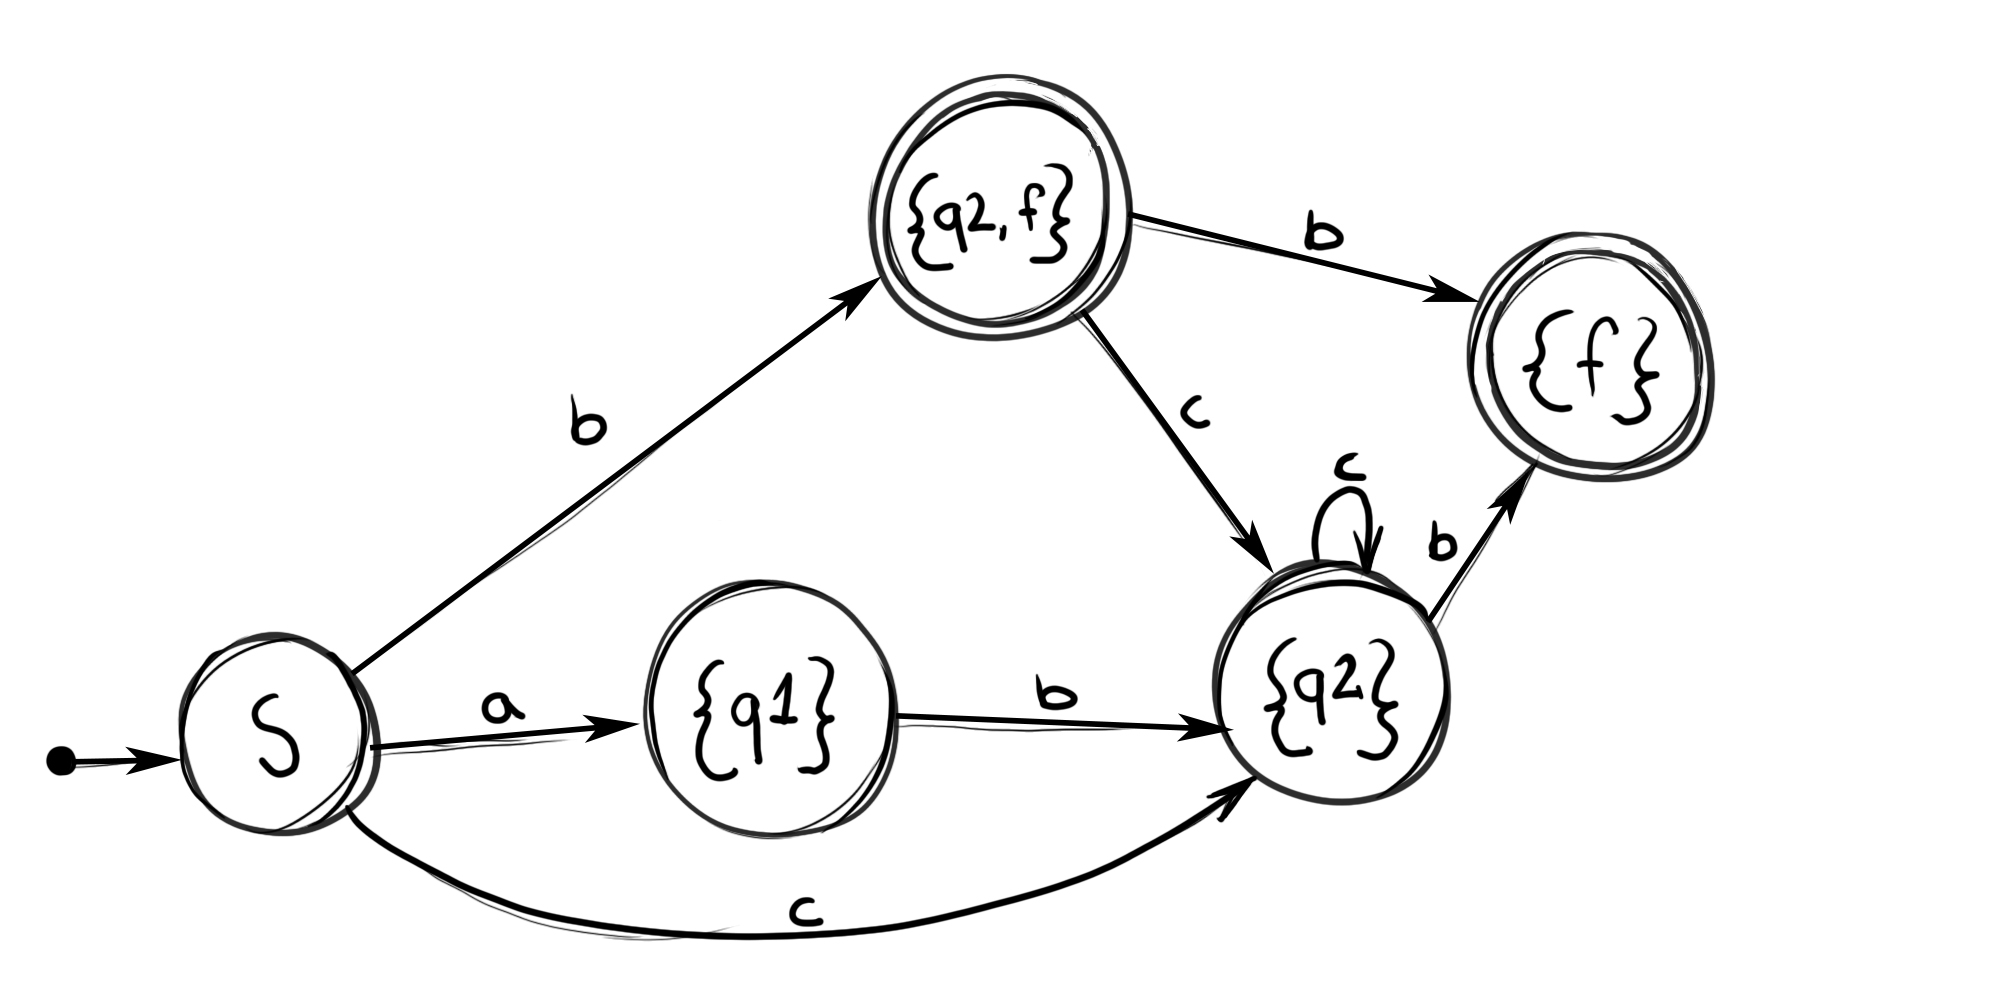
\includegraphics[scale=0.25]{dfa}
\end{figure}


Ein Token ist ein Baustein, ein Zeichen oder Wort dessen einzelne syntaktische Bedeutung wir kennen. Der Gesamtkontext, also die semantische Bedeutung des
vom Nutzer geschriebenen Programm erschliesst sich uns damit zum aktuellen Zeitpunkt allerdings noch nicht.

\newpage
\section{Der Baum der Erkenntnis}

Daf\"ur m\"ussen wir weitere Transformationen am Quelltext des Nutzers
vornehmen. Der Parser ist dabei der Teil eines Compilers welcher
entscheidet ob ein Satz in der Quellsprache den formalen Syntaxregeln dieser entspricht. Er erkennt also fehlerhafte Syntax und gibt dem Nutzer Feedback in Form von
Fehlermeldungen, \"uber die k\"onnen Sie in Torbens Abschnitt mehr erfahren.
Aber warum brauchen wir \"uberhaupt noch einen Schritt k\"onnen wir nicht
Regul\"are Ausdr\"ucke verwenden um auch diesen Teil der Sprachsyntax zu
definieren? Wir wollen dies Anhand folgenden mathematischen Ausdrucks betrachten.

\begin{equation}
    42 + foo * 2
\end{equation}

Mit Leichtigkeit k\"onnen wir eine formale Spezifikation einer Sprache finden
welche diese Art mathematischer Ausdr\"ucke akzeptiert. Leider geben uns regul\"are Ausdrucke nicht genug macht um Vorrangsbah\"anigkeiten zu beachten.
Wir brauchen also ein anderes Werkzeug, welches uns erm\"oglicht eine Definition
einer anderen, maechtigeren formalen Sprache zu erstellen. Im Gegensatz zu einer formalen Sprache
f\"ur Lexer definition muss sie die M\"oglichkeit besitzen Parsepriorit\"aten auszudr\"ucken.
Dem Lexer ist nicht klar welche Version des erzeugten Syntaxbaumes korrekt ist, nur mit einer regul\"aren Sprache nicht die M\"oglichkeit haben das Konzept von Punktrechnung vor Strichrechnung auszudr\"ucken.
\begin{figure}[h]
    \centering
    \subfloat[Mit Ber\"ucksichtigung von Operatorvorrang]{{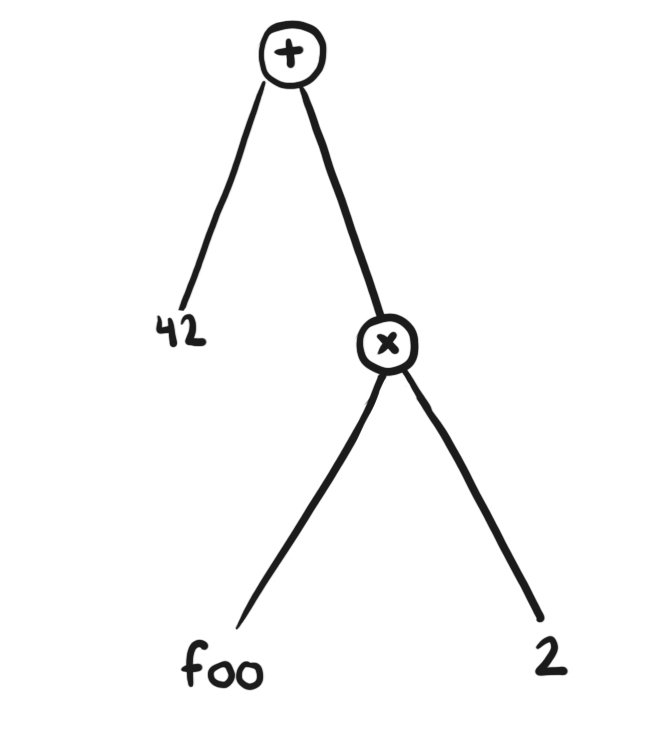
\includegraphics[width=5cm]{astright} }}%
    \qquad
    \subfloat[Ohne Ber\"ucksichtigung von Operatorvorrang]{{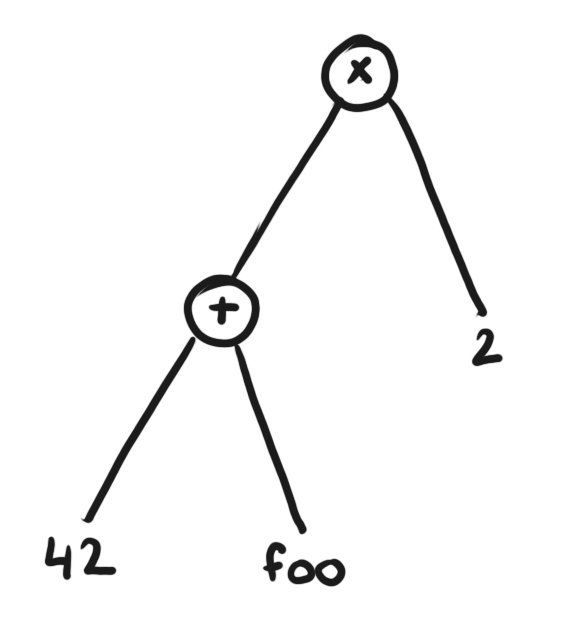
\includegraphics[width=5cm]{astwrong} }}%
    \label{fig:vs}%
\end{figure}

Diese formale Defintion k\"onnen wir dann mithilfe weiterer Werkzeuge, die wohl bekanntesten dieser Art sind Flex und Bison, daher auch die \"Uberschrift,
automatisiert in die Implementierung eines Parsers generieren welcher den formalen Anforderungen unserer Sprache entspricht. Wir
haben uns im Zuge unseren Projektes allerdings gegen den Einsatz einer solchen formalen Defintion in Zusammenarbeit mit einem Parsergeneratorsystem wie Bison
und Flex entschieden.
Hauptgrund f\"ur diese Entscheidung waren massgeblich die Fehlermeldungen, welche wir als essentiellen Bestandteil einer Anf\"angerfreundlichen Programmiersprache identifiziert haben. Dadurch dass wir unserer Lexer und Parser ohne Zuhilfenahme externer Codegenerationswerkzeuge
geschrieben haben, besitzen wir auch die volle Kontrolle \"uber die Generation
und Ausgabe der entstehenden Fehlermeldungen.
Allerdings haben an an dieser Stelle aber auch die Probleme angefangen. Da
wir uns nicht auf externe Werkzeuge verlassen konnten, kam nat\"urlich die
Frage auf: “Wie schreibe ich einen eigenen Parser?”. Wie sich herausstellte
gibt nicht einen Algorithmus den es zu implementieren gilt um eine Parser zu
programmieren, sondern sehr viele verschiedene, einer schwieriger und komplexer als der andere. Die Fachliteratur f\"ur dieses Thema besch\"aftigt sich
vielmehr mit den verschiedenen M\"oglichkeiten der Parsergeneration, also wie von
einer oben beschrieben formalen Defintion automatisch ein korrekter Parser f\"ur eben
diese Spezifikation generiert werden kann, anstatt wie man selbst, von Hand, einen solchen Parser implementiert.
Abgeschreckt davor einen Shift-Reduce Parser schreiben zu m\"ussen, haben
wir dann gl\"ucklicherweise “Recurssive descent parsing” zu Deutsch also “Rekursives Abstiegsparsen” entdeckt. Ein Rekursiver Abstiergsparser gilt als besonders einfach von Hand zu implementieren \footcite{recdec} was auch der Grund daf\"ur ist weshalb wir im STGI Compiler auf dieses Verfahren setzen.

\begin{figure}[h]
\caption{Beispiel f\"ur eine formale Defintion zum Aufbau einer Funktion,
in erweiterter Backaus-Naur-Form}
\setlength{\grammarparsep}{20pt plus 1pt minus 1pt}
\setlength{\grammarindent}{12em}

\begin{grammar}
<Funktion> ::= <Ident> ':=' 'fun' '(' Parameterliste ')' -> <Typ> <Block>

<Block> ::= <Stmt> | <Block> ';' , <Stmt>

<ParameterListe> ::= <Parameter> | <ParameterListe> , <Parameter>

<Parameter> ::= <Ident> ':' <Datentyp>

<DatenTyp> ::= Zahl
\alt{Text}
\alt{Bool}
\alt{Ident}
\end{grammar}
\end{figure}

\subsection{Mit Rekursion bis nach ganz unten}

Beim Rekursiven Abstiegsparsen wird der Parser \"ahnlich wie der Lexer als
simpler Zustandsautomat modeliert und der \"Ubergang zwischen den Zust\"anden wird durch rekursiv definierte Teilparser implementiert. Dies entspricht zu grossen Teilen der rekurssiv definierten Grammatikspezifikation unserer Sprache.
Betrachten wir nochmal das Beispiel von oben. Wenn Sie eine Funktionssignatur parsen
wollen k\"onnen Sie diese in kleinere Bausteine zerlegen. Jeder dieser Bausteine kann
dann entweder wiederum selbst in noch kleinere Bestandteile zerlegt werden
oder es ergibt sich ein, meist so einfaches Muster welches wiederum problemslos als simplen DFA implemtiert werden kann.
\begin{figure}[h]
    \emph{foo := fun(a: Zahl, b: Zahl) -> Text{}}
\end{figure}
Um einen Parser f\"ur die obige Funktion foo zu schreiben zerlegen wir diese
also in 2 Bestandteile: Den Funktionskopf und den Funktionsk\"orper. Laut unserer Sprachsyntax muss auf den Namen der Funktion, das defintionszeichen
“:=” folgen, auf dieses wiederum folgt das Funktionsschl\"usselwort gefolgt von
einer \"offnenden runden Klammer die, mit einer schliessenden Runden Klammer, die durch jeweils ein Komma getrennte Liste der Parameter begrenzt. Ein
Parameter setzt sich dabei nach dem Muster “name: Datentyp” zusammen, wir
k\"onnen also eine seperate Funktion schreiben um Parameter zu parsen. Diese
wiederum erwartet den Namen des Parameters und ruft dann die Funktions
zum parsen eines Datentypen auf. Sobald wir eine schliessende Runde Klammer finden h\"oren wir auf parameter zu parsen und erwarten statdessen eine
\"offnende Geschweifte Klammer f\"ur den K\"orper der Funktions. Dieser setzt
sich wiederum aus den einzelnen Statements zusammen.
In Pseudocode k\"onnte eine Funktions zum parsen der obigen Funktionsdeclaration wie folgt aussehen.

\begin{figure}[h]
    \caption{Beispielimplementierung einer Funktion um Funktionsdefinitionen zu parsen}
  \begin{minted}{c}
    def parseFunktion():
        erwarte(FUN)
         name := erwarte(Ident)
         parameter := []
         solange naechsterToken() != RParen:
                parameter.fuegeHinzu(parseParameter())
                erwarte(KOMMA)
    koerper := parseBlock()
  \end{minted}
\end{figure}

\subsection{Typeinference (Typenableitung)}
Eine der ersten Entscheidungen die wir beim Konzepieren von STGI getroffen
haben war, unsere Sprache mit einem statischem Typenchecker zu versehen.
D.h.alle Datentypen werden zur Kompilierzeit, was im Gegensatz zu einer
dynamisch gecheckten Sprache steht, vom Kompiler \"uberpr\"uft. Die Entscheidung zwischen einer statischen versus einer dynamischen Typenanalyse geh\"ort
zu den gr\"ossten Designentscheidungen die bei der Entwicklung einer eigenen
Programmiersprache getroffen werden k\"onnen. Anh\"anger dynamischer Sprachen, haben
daf\"ur z.B. den Vorteil sich keine Gedanken \"uber Datentypen beim Schreiben eines Programmes machen zu m\"ussen und solange der Compiler irgendwie vom gegebenen Datentyp auf den geforderten umwandeln kann, passiert dies auch ohne ein explizites Zutun des Nutzers. Dies erlaubt h\"aufig k\"urzere
Entwicklungszeiten, weil die Datentypen eben zur Zeit der Entwicklung nicht ber\"ucksichtigt werden m\"ussen.
Studien haben allerdings gezeigt dass besonders f\"ur komplexe Aufgaben und tieferes Verst\"andnis einer Programmschnittstelle geht, statisch typisierte Sprachen helfen ein Programm zu verstehen. \footcite[vgl.][694-695]{svd}

Dies ist aus zweierlei Gr\"unden f\"ur den Nutzer expliziet mit einem Blick auf
unsere Zielgruppe von Anf\"angern wichtig.
\begin{itemize}
\item{Fr\"uhe Fehler ergeben f\"ur den Nutzer ein viel besseres Feedback: Er
muss sein Programm nicht vollst\"andig ausf\"uhren um zu erfahren ob er
einen Fehler behoben hat.}
\item{Sie erm\"oglicht unter dem Aspekt der formalen Anlyse eine Aussage
\"uber die Korrektheit eines Programms zu treffen.}
\end{itemize}

Besonders deutlich kann dies an folgenden Beispiel aufgezeigt werden:
\begin{figure}[h]
\caption{Beispiel expliziete vs implizierte Typenangabe}
\begin{minted}{c}
// ohne Typenableitung
foo :[(Zahl, Zahl, Zahl)]= [(1, 2, 3), (4, 5, 6), (7, 8, 9)]
// Compiler leitet den Typ selbst ab
foo := [(1, 2, 3), (4, 5, 6), (7, 8, 9)]
\end{minted}
\end{figure}

Hier sticht allerdings die Verbosit\"at den Datentyp, f\"ur jeden Variable eines
Programms, angeben zu m\"ussen ins Auge. Zusammen mit dem Argument der
schnelleren Entwicklungszeit wie diese h\"aufig bei bei Anwendern dynamischen Programmiersprachen gelobt werden, haben wir uns dann f\"ur einen Hybridansatz der automatisierten Typenableitung entschieden. Das heisst der Compiler \"uperpr\"uft
zwar immer noch w\"ahrend der Kompilierzeit alle Typenabh\"anigkeiten, ist allerdings intelligent genug, sich die n\"otigen und angegebenen Datentypen ohne
zutun des Nutzers abzuleiten.

\"Ahnlich wie beim Parsen gibt es auch f\"ur die Typenableitung verschiedene
Anforderungen und somit auch verschiedene Ans\"atze. Allerdings haben wir
schnell herausgefunden, dass das ``defacto goto'' Verfahren f\"ur Typenableitung
auf einem Algorithmus von “Hindley und Milner” beruht. Im folgenden Abschnitt werden wir uns also der Typenableitung nach HM widmen.

\subsection{Typenableitung nach Hindley und Milner}
Wir werden uns im Zuge dieser Ausarbeitung die feine formalen Aspekte der
theoretischen Typenableitung sparen, da dies die Grenzen dieses Projektes bei weitem sprengen w\"urde.
Statdessen wollen wir Typenableitung an einigen praktischen Beispiel
erkl\"aren:
\begin{figure}[h]
  \caption{Beispiel Einschraenkung durch Verwendung in Ausdruck}
  \begin{minted}{c}
    // Einschr\"ankung: *: Zahl => Zahl
    foo := x * 2
  \end{minted}
\end{figure}

\begin{figure}[h]
  \caption{Beispiel Einschraenkung durch Verwendung in Statement}
  \begin{minted}{c}
    // Einschr\"ankung: Bedinung: Bool
    wenn foo dann {
      //...
    }
  \end{minted}
\end{figure}

\begin{figure}[h]
  \caption{Beispiel Einschraenkung durch Verwendung im Kontex eines Statements}
  \begin{minted}{c}
    // Einschr\"ankung: Bedinung: Bool
    wenn foo dann {
      //...
    }
  \end{minted}
\end{figure}

Wie Sie den vorhergehenden Beispielen entnehmen konnten, spielt der Kontex um einen Ausdruck eine wichtige Rolle um dessen Typ zu bestimmen.
Durch ihn erhalten wir Einschr\"akungen \"uber den Typ eines
Ausdrucks. So wissen wir z.B. dass im 1. Beispiel ``foo'' den gleichen Wert wie $x * 2$ annehmen muss, desweitern dass es sich bei dem Typ von $x$ um Zahl handeln muss, da wir es sonst nicht mit $2$ mulitplizieren k\"onnten. Nachdem wir diese Einschr\"ankungen gesammelt haben, versuchen wir mit einem Unifikationsalgorithmus einen Beweis
oder eine L\"osung zu finden die alle Einschr\"ankungen erf\"ullt \footcite[vgl.][44]{mgordon}. K\"onnen wir eine
solche L\"osung nicht finden, also wenn sich die Einschr\"ankungen gegenseitig
widersprechen, haben wir einen Typenfehler gefunden.

Konkret gehen wir also in einem ersten Schritt durch unsere Beispielsfunktion und ersetzen s\"amtliche
Typen, die bis jetzt nur einen Platzhalterwert besitzen durch eine Typenvariable,
Typenvariablen sind auch Platzhalter die wir ein zu einem sp\"aternen Schritt durch tats\"achlichen Typen im Syntaxbaum ersetzen. \footcite{tbe}

\begin{figure}[h]
  \caption{Beispiel Einschr\"ankung durch Verwendung in Statement}
  \begin{minted}{c}
    foo := feld(von: Zahl<0, bis: Zahl<1>) -> [Zahl]<2> {
      zahlen : <3> = []
      fuer i :<4> = 0..10: <5> {
        b[i] = i
      }
      rueckgabe zahlen<6>
    }
  \end{minted}
\end{figure}

Mit diesem Platzhaltern k\"onnen wir nun folgende “Einschr\"ankungen” formulieren welche f\"ur Typen in unserer Funktion zutreffen m\"ussen.
\begin{itemize}
  \item{<0> = Zahl}
  \item{<1> = Zahl}
  \item{<2> = [Zahl]}
  \item{<3> = <4>}
  \item{<4> = <5>}
  \item{<5> = [Zahl]}
\end{itemize}

\pagebreak
Im n\"achsten Schritt werden die verschiedenen Einschr\"ankungen durch Unifikation gel\"ost. Unifikation beschreibt eine Vorangehensweise zur Vereinheitlichung logischer Ausdrücke. Zwei Ausdrücke werden unifiziert, indem ihre Variablen
so durch geeignete Terme ersetzt werden und substituiert, dass die resultierenden Ausdrücke gleich sind. \footcite{unidef} So erhalten wir schlussendlich folgende Substituion. \footcite{tbe}
\begin{itemize}
  \item{<0> = Zahl}
  \item{<1> = Zahl}
  \item{<2> = [Zahl]}
  \item{<3> = [Zahl]}
  \item{<4> = Zahl}
  \item{<5> = [Zahl]}
\end{itemize}
Im letzen Schritt werden dann die zuvor in den Syntaxbaum eingef\"ugten
Platzhalter durch die richtigen Datentypen ersetzt.


\section{Wirklich ein Compiler?}
Bisher haben wir immer in dieser Ausarbeitung immer von einem Compiler
gesprochen. Dies entspricht allerdings nicht der vollen Wahrheit. Ein Compiler beschreibt den spezifischen Vorgang, \"ahnlich einem \"Ubersetzter, von
einer Sprache in eine andere zu \"ubersetzen. Urspr\"unglich haben wir das
auch geplant. Bez\"uglich diesem Plan hat sich w\"ahrend des Projektes wohl
am meisten ge\"andert. Der erste Plan war von STGI auf C++ zu \"ubersetzen, die allererste Version des Compilers hat auch genau das gemacht. Wir
haben diesen Ansatz allerdings wieder verworfen ein Grund daf\"ur war die
schlechte Unterst\"uztung von “Buildsystem” f\"ur C++. Jemand der gerade
erst mit dem Programmieren anf\"angt, kann keine komplizierte Installation eines C++ Compilers zugemutet werden. Wie sich herausstellte ist es notorisch
schwierig C++ Projekte auf Windows mit all den ben\"otigten Bibilotheken
und Abh\"anigkeiten zu kompilieren. Verh\"artet kam dann noch die Bruchst\"uckhafte C++ Kenntnis der Gruppe zu tragen. Wir haben dann noch ein paar
weitere Versuche unternommen anstatt auf C++ auf C zu kompilieren. Nach
einigen kleinen Versuchen stellte sich dann aber zugleich heraus dass wir noch
weniger C Kentnisse wie zuvor C++ hatten. Wir wussten einfach nicht wie
wir bestimmte Features unserer Hochsprache in C welches bekannt daf\"ur ist
sehr nahe an der Maschine zu operieren sollten.
Schlussendlich haben wir noch die M\"oglichkeiten des LLVM Frameworks evaluiert waren aber abgeschreckt von der veralteten Dokumentation und den
komplizierten Schnittstellen von LLVM.

\subsection{Wir schreiben einen Interpreter}
Mit dem Wechsel zu Rust haben wir uns dann aber entg\"ultig dazu entschlossen den Gedanken der
kompilation auf eine andere Hochsprache komplett zu verwerfen und stattdessen einen Interpreter zu schreiben.
Aber wie f\"urt ein Computer so ein vom Benutzer geschriebenes Programm
eigentlich aus? Zu diesem Zeitpunkt haben wir es bereits in seine atomare
Bestandteile (Tokens), deren Bedeutung und Funktion w\"ahrend dem
Parsen verstanden und in einen Syntaxbaum umgewandelt danach noch fehlende
Datentypen f\"ur den Benutzer erg\"anzt, aber wie f\"uhren wir das Programm
welches der Benutzer geschrieben hat tats\"achlich aus?
Wie oben beschrieben wird hier der Syntaxbaum und die Position der Knotenpunkte untereinander besonders wichtig.
Um den erzeugten Syntaxbaum zu interpretieren. Gehen wir von unten nach oben durch alle Knoten und ersezten jeweils den Elternknoten durch das Ergebnis der Kinderknoten.
\begin{figure}[h]
\caption{Beispiel eines mathematischen Ausdrucks als Syntaxbaum. Um ihn zu interpretieren berechnen wir erst foo * 2 um dann dieses Ergebnis auf 42 zu addieren}
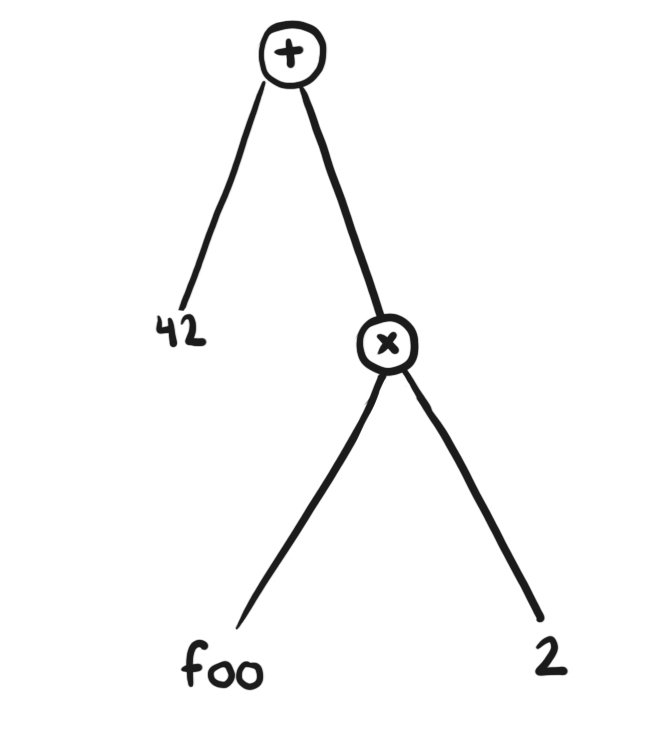
\includegraphics[scale=0.2]{astright}
\end{figure}

\newpage
\section{Einige Reflektionen \"uber den Seminarkurs}
Aller Anfang ist schwer und so war es auch f\"ur uns nicht leicht ein passendes Projekt zu finden. Von 3D Scanner zu T\"urschloss mit automatischer
Gesichtserkennung stand alles im Raum. Schlussendlich hat sich dann die Gelegenheit ergeben eine eigene Programmiersprache zu entwickeln, speziell um
Leuten wie sie jedes Jahr unser Schulhaus betreten um ihren Platz in der 11.
Klasse einnehmen, helfen den Einstieg ins Programmieren zu erleichtern. Ich
war sofort Feuer und Flamme von der Idee, sie schien mir anspruchsvoll und
spannend zugleich. Postwendend kann ich sagen dass sich diese Erwartungen
mehr als bewahrheitet haben. So stark bewahrheitet dass aus anspruchsvoll,
zu anspruchsvoll und aus spannend pure verzweiflung wurde, wenn der eigene Compiler mal wieder nicht das tut was er soll. Naja zumindest wusste ich dann wer daran Schuld hat. Frustrierend war vor allem der dicke akademische Vorhang der vor vielen Themen hing und sich anf\"uhlte als w\"are er
kaum zu durchdringen. Viele Bereiche beim programmieren eines Compilers,
wie etwa Parser oder Typenableitung sind mit jahrzehntelanger Forschung auf
ihrem jeweiligen Gebiet verbunden. Entsprechend viel Formalismus existiert zu
diesen Gebieten und so kann es sich manchmal wie viel zu dichtes Unterholz
anf\"uhlen durch das man kriechen muss um an die Leckeren Beeren zu komemn. Oft hat sich nach anf\"anglicher Recherche und Panik bei dem Umfang
eines Themas herausgestellt dass der Kern der Sache gar nicht so schwierig ist
wie anfangs angenommen. Trotzdem hat sich jedes Modul angef\"uhlt wie eine
Bergbesteigung. Das Projekt hat mir pers\"onlich sehr viel Spass gemacht.
Ich denke trotzdem dass es, schon aufgrund der Unmengen an Formalismus in der Fachliteratur, kein geignetes Projekt f\"ur 3 Programmiereinsteiger in der Eingangsklasse ist.
Besonders belohnend war in Folge dessen dann aber auch jedes mal die Aussicht vom Gipfel des Berges.

\newpage
\section{Erklärung der Urheberschaft}

Ich erkläre hiermit an Eides statt, dass ich die vorliegende Arbeit
ohne Hilfe Dritter und ohne Benutzung anderer als der angegebenen
Hilfsmittel angefertigt habe; die aus fremden Quellen direkt oder
indirekt übernommenen Gedanken sind als solche kenntlich gemacht. Die
Arbeit wurde bisher in gleicher oder ähnlicher Form in keiner anderen
Prüfungsbehörde vorgelegt und auch noch nicht veröffentlicht.

\vspace{4cm}

\hspace{2cm} Ort, Datum \hfill Unterschrift \hspace{2cm}
\newpage
\printbibliography
\nocite{*}

\end{document}
